\section{Introducción}
Los pronósticos de CPU y memoria pueden aportar información a la planificación de capacidad y al autoescalado de microservicios. Una arquitectura de microservicios distribuye funcionalidades entre componentes que se comunican mediante llamadas; sus mediciones temporales y relaciones permiten estudiar tanto la historia local como información del entorno. Sin embargo, pronosticar el uso registrado no equivale a estimar demanda sin restricciones ni demuestra que un controlador asigne mejor los recursos. Los trabajos sobre aprendizaje de cargas, autoescalado y pronóstico de recursos ofrecen el contexto aplicado \cite{powerprediction,autoscaling2025,temposcale,aero}. Este estudio evalúa errores puntuales y ejecución de modelos, sin medir energía, facturación o cumplimiento de acuerdos de servicio.

La telemetría puede faltar cuando fallan la recolección, el transporte o los servicios. El predictor debe distinguir el último valor conocido de una medición nueva. El problema inicial fue modificar un modelo ligero para representar esa procedencia y cambiar su descomposición temporal. Un escalar imputado permite ejecutar el modelo, pero no identifica el proceso de observación. Añadir características de ausencia puede ayudar a interpretar la historia y también incrementar capacidad, redundancia o ajuste al generador sintético. Su utilidad requiere evidencia de error y coste, no solamente una justificación semántica.

DLinear combina proyecciones afines de una componente móvil y su residual \cite{dlinear}. Cuando el suavizamiento es una transformación lineal fija, la suma sigue siendo una función afín de la ventana. Reducir su parametrización no crea necesariamente una nueva clase funcional. El suavizamiento dependiente de disponibilidad y las características explícitas de ausencia constituyen intervenciones distintas. Ni una equivalencia algebraica ni un menor número de parámetros garantizan mejorar la predicción. Esta distinción motivó pasar del estudio de descomposición a modelos compactos y, después, a referencias más amplias.

La investigación integra cinco fases complementarias. La fase I evalúa E0--E5 y comparadores originales sobre 28 servicios de ChronoGraph. La fase II estudia C0--C3 y la regla V2 seleccionada mediante validación, sobre la misma prueba conocida. La fase III vuelve a ajustar modelos fuente con el protocolo ampliado y los transfiere a 32 servicios adicionales. La fase IV añade mecanismos de pérdida, horizontes directos, ventanas y un caso externo de Alibaba 2022. La fase V mide el coste de las implementaciones. La secuencia desarrolla una pregunta común; las fases no son réplicas independientes ni sus errores se suman.

El resultado histórico favorable de E5 en memoria motivó desarrollos posteriores. Los cuatro contrastes principales se congelaron localmente antes de evaluar los servicios destino, aunque el período fuente ya era conocido. Los servicios adicionales comparten infraestructura y período con la fuente: constituyen transferencia espacial calibrada, no una replicación temporal cegada. Los protocolos y pesos congelados mejoran la transparencia del procedimiento, pero no convierten toda la investigación en un ensayo prospectivo independiente ni equivalen a un prerregistro público.

La brecha abordada es una evaluación conjunta y trazable de descomposición, procedencia de mediciones, capacidad, coste y transferencia. La contribución es empírica: una parametrización afín compacta con dos descriptores separados, comparación emparejada de quince familias bajo diez condiciones, extensiones de horizonte y ventana, transferencia externa calibrada, reconstrucción de métricas y mediciones de inferencia CPU/CUDA. Se conservan resultados negativos y cambios de clasificación. La contribución no consiste en afirmar que una arquitectura resuelve universalmente la gestión de recursos.

\subsection{Preguntas de investigación y alcance}
La pregunta central es cómo afectan la descomposición temporal, la representación de telemetría incompleta y la complejidad a precisión, robustez, eficiencia y transferencia del pronóstico. Se concreta en seis preguntas: PI 1, cómo cambia el error al perder observaciones; PI 2, qué compromiso produce la descomposición fija, el suavizamiento dependiente de disponibilidad y la parametrización compacta; PI 3, cuándo ayudan la fracción ausente y la edad; PI 4, si un modelo afín compacto conserva precisión con menos parámetros; PI 5, cómo cambian las conclusiones entre servicios, horizontes y dominios; y PI 6, cuánta variación aparece entre inicializaciones, máscaras y períodos.

La hipótesis principal compara A3 con DLinear y E5 para CPU y memoria mediante cuatro contrastes bilaterales. La finalización no exige obtener una mejora. La monotonía frente a pérdidas, las ablaciones, mecanismos añadidos, ventanas, horizontes y transferencia externa son análisis secundarios descriptivos. La evidencia histórica es exploratoria y genera hipótesis. Un efecto puede conservar dirección entre inicializaciones y concentrarse en pocos servicios, por lo que consistencia entre semillas, portabilidad y tamaño del modelo se interpretan separadamente. La Fig.~\ref{fig:flow} muestra el flujo de selección y evaluación.
\begin{figure*}[!t]\centering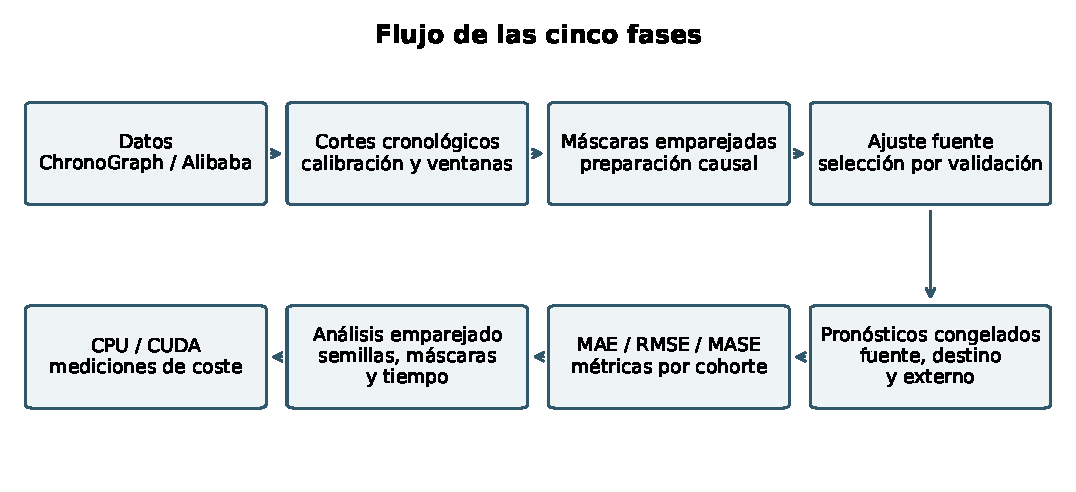
\includegraphics[width=0.93\textwidth]{figuras/es_01_methodology.pdf}
\caption{Flujo experimental. La selección y los pesos usan entrenamiento y validación de los 28 servicios fuente. Los 32 servicios destino aportan estadísticas de calibración del prefijo, sin ajuste de pesos. Alibaba utiliza un prefijo separado de seis horas.}\label{fig:flow}
\end{figure*}
